\documentclass[aspectratio=169]{beamer}

% Theme and colors
\usetheme{Madrid}
\usecolortheme{whale}
% Custom colors
\definecolor{primary}{RGB}{41, 128, 185}
\definecolor{secondary}{RGB}{52, 152, 219}
\definecolor{accent}{RGB}{231, 76, 60}
\definecolor{lightgray}{RGB}{236, 240, 241}

% Packages
\usepackage[utf8]{inputenc}
\usepackage{graphicx}
\usepackage{amsmath}
\usepackage{amsfonts}
\usepackage{amssymb}
\usepackage{mathpazo} % Palatino font
\usepackage{multirow}
\usepackage{tcolorbox}
\usepackage{tikz} % For diagrams
\usepackage{caption} % For figure captions
\usepackage{adjustbox} % For adjusting box
\usepackage{float} % For better float control

% Beamer specific configurations
\setbeamercolor{structure}{fg=primary}
\setbeamercolor{background canvas}{bg=white}
\setbeamercolor{normal text}{fg=black}

% Information for the title page
\title{Lesson 5: Graphing Quadratic Functions in APQ Form}
\author{Yi-Chen Lin}
\date{June 10, 2025}

\begin{document}

% Title page
\begin{frame}
    \titlepage
\end{frame}

% Table of Contents
\begin{frame}{Table of Contents}
    \tableofcontents
\end{frame}

% Section I: Quadratic Functions in Different Forms
\section{Quadratic Functions in Different Forms}

\begin{frame}{I) Quadratic Functions Written in Two Different Forms - Part 1}
    \begin{tcolorbox}[colback=lightgray,colframe=primary,title=Key Forms]
        \footnotesize
        \begin{itemize}
            \item \textbf{General Form:}
                \[ y = ax^2 + bx + c \]
                \begin{itemize}
                    \item Axis of Symmetry: $x = \frac{-b}{2a}$
                    \item Y-intercept: $(0,c)$
                    \item Not as easy finding the vertex
                \end{itemize}
        \end{itemize}
    \end{tcolorbox}
\end{frame}

\begin{frame}{I) Quadratic Functions Written in Two Different Forms - Part 2}
    \begin{tcolorbox}[colback=lightgray,colframe=primary,title=Key Forms (Cont.)]
        \footnotesize
        \begin{itemize}
            \item \textbf{Vertex Form (APQ form):}
                \[ y = a(x-p)^2 + q \]
                \begin{itemize}
                    \item Finding the vertex is very easy!!
                    \item Graphing in APQ form is also easy
                    \item All you need to do is find the constants "$a$", "$p$", and "$q$"
                    \item Vertex: $(p,q)$
                    \item AOS: $x = p$
                \end{itemize}
        \end{itemize}
    \end{tcolorbox}
\end{frame}

\begin{frame}{Example: Identifying Constants in APQ Form}
    \begin{tcolorbox}[colback=lightgray,colframe=primary,title=Example]
        \footnotesize
        For the equation $y = 3(x-2)^2 + 7$:
        \begin{itemize}
            \item $a = 3$
            \item $p = 2$
            \item $q = 7$
            \item Vertex: $(2,7)$
            \item AOS: $x = 2$
        \end{itemize}
    \end{tcolorbox}
\end{frame}

\begin{frame}{Example Graph: $y = 3(x-2)^2 + 7$}
    \begin{figure}[H]
        \centering
        \includegraphics[width=0.6\textwidth]{e1.png}
        \caption{Example graph illustrating constants in APQ form for $y = 3(x-2)^2 + 7$.}
    \end{figure}
\end{frame}

% Section II: Graphing Quadratic Functions
\section{Graphing Quadratic Functions}

\begin{frame}{II) Graphing Quadratic Functions in APQ Form}
    \begin{tcolorbox}[colback=lightgray,colframe=primary,title=Key Points]
        \footnotesize
        \begin{itemize}
            \item A Quadratic function in vertex form is much easier to graph
            \item Using constants "$a$", "$p$", \& "$q$", we can find:
                \begin{itemize}
                    \item Vertex: $(p,q)$
                    \item Domain: $x \in \mathbb{R}$
                    \item Axis of Symmetry: $x = p$
                    \item Range: $y \geq q$ or $y \leq q$
                    \item Y-intercept: make $x=0$, solve for $y$
                    \item X-intercept: make $y=0$, solve for $x$
                \end{itemize}
        \end{itemize}
    \end{tcolorbox}
\end{frame}

% Section II.5: Formula and Graph Ideas
\subsection{Formula and Graph Ideas}

\begin{frame}{II.5) Understanding the Formula $y = a(x-p)^2 + q$ - Part 1}
    \begin{tcolorbox}[colback=lightgray,colframe=primary,title=Formula Components]
        \footnotesize
        \begin{itemize}
            \item \textbf{Basic Formula:} $y = a(x-p)^2 + q$
            \item \textbf{Each constant has a specific effect:}
        \end{itemize}
    \end{tcolorbox}
\end{frame}

\begin{frame}{II.5) Understanding the Formula $y = a(x-p)^2 + q$ - Part 2}
    \begin{tcolorbox}[colback=lightgray,colframe=primary,title=Constant Effects (Cont.)]
        \footnotesize
        \begin{itemize}
            \item $a$: Controls the shape and direction
                \begin{itemize}
                    \item If $a > 0$: Parabola opens up
                    \item If $a < 0$: Parabola opens down
                    \item Larger $|a|$: Narrower parabola
                    \item Smaller $|a|$: Wider parabola
                \end{itemize}
            \item $p$: Controls horizontal position
                \begin{itemize}
                    \item Moves vertex left/right
                    \item Positive $p$: Shift right
                    \item Negative $p$: Shift left
                \end{itemize}
            \item $q$: Controls vertical position
                \begin{itemize}
                    \item Moves vertex up/down
                    \item Positive $q$: Shift up
                    \item Negative $q$: Shift down
                \end{itemize}
        \end{itemize}
    \end{tcolorbox}
\end{frame}

\begin{frame}{Graph Ideas and Key Points}
    \begin{tcolorbox}[colback=lightgray,colframe=primary,title=Graphing Strategy]
        \footnotesize
        \begin{itemize}
            \item \textbf{Step 1:} Identify the vertex $(p,q)$
            \item \textbf{Step 2:} Draw the axis of symmetry $x = p$
            \item \textbf{Step 3:} Use the value of $a$ to determine:
                \begin{itemize}
                    \item Direction of opening
                    \item Width of parabola
                    \item Pattern of points
                \end{itemize}
            \item \textbf{Step 4:} Plot points using the pattern:
                \begin{itemize}
                    \item For $a=1$: 1, 3, 5, 7, ...
                    \item For $a=2$: 2, 6, 10, 14, ...
                    \item For $a=3$: 3, 9, 15, 21, ...
                \end{itemize}
            \item \textbf{Step 5:} Connect points to form parabola
        \end{itemize}
    \end{tcolorbox}
\end{frame}

\begin{frame}{Example: Complete Analysis - Part 1}
    \begin{tcolorbox}[colback=lightgray,colframe=primary,title=Example: y]
        \footnotesize
        \begin{itemize}
            \item Equation: $y = 2(x-3)^2 - 5$
            \item \textbf{Constants:}
                \begin{itemize}
                    \item $a = 2$ (opens up, medium width)
                    \item $p = 3$ (shifts right 3 units)
                    \item $q = -5$ (shifts down 5 units)
                \end{itemize}
            \item \textbf{Key Features:}
                \begin{itemize}
                    \item Vertex: $(3,-5)$
                    \item Axis of Symmetry: $x = 3$
                    \item Pattern: 2, 6, 10, 14, ...
                \end{itemize}
        \end{itemize}
    \end{tcolorbox}
\end{frame}

\begin{frame}{Example: Complete Analysis - Part 2}
    \begin{tcolorbox}[colback=lightgray,colframe=primary,title=Example: $y = 2(x-3)^2 - 5$ (Graphing)]
        \footnotesize
        \begin{itemize}
            \item \textbf{Graphing Steps:}
                \begin{enumerate}
                    \item Plot vertex at $(3,-5)$
                    \item Draw AOS at $x = 3$
                    \item Move right 1 unit, up 2 units
                    \item Move right 1 more unit, up 6 more units
                    \item Continue pattern
                    \item Mirror points across AOS
                \end{enumerate}
        \end{itemize}
    \end{tcolorbox}
\end{frame}

\begin{frame}{Example Graph: Graphing $y = 2(x-3)^2 - 5$}
    \begin{figure}[H]
        \centering
        \includegraphics[width=0.6\textwidth]{e2.png}
        \caption{A visual representation of the graphing steps for $y = 2(x-3)^2 - 5$, showing the vertex, axis of symmetry, and parabolic shape.}
    \end{figure}
\end{frame}

% Section III: Horizontal Translations
\section{Horizontal Translations}

\begin{frame}{III) Horizontal Translations}
    \begin{tcolorbox}[colback=lightgray,colframe=primary,title=Key Concepts]
        \footnotesize
        \begin{itemize}
            \item A parabola will shift left or right depending on the constant "$p$" that is placed inside the brackets with "$x$"
            \item Look inside the brackets to find what the value of "$p$" is
            \item When $p=0$, the graph is centered on the Y-axis
            \item When $p>0$, the graph shifts right
            \item When $p<0$, the graph shifts left
        \end{itemize}
    \end{tcolorbox}
\end{frame}

% Section IV: Vertical Translations
\section{Vertical Translations}

\begin{frame}{IV) Vertical Translations (VT)}
    \begin{tcolorbox}[colback=lightgray,colframe=primary,title=Key Concepts]
        \footnotesize
        \begin{itemize}
            \item A Vertical shift (UP or Down) will occur if a constant is added to the equation outside of the brackets
            \item The value of "$x$" is squared first and then we add/subtract the constant
            \item When $q>0$, the graph shifts up
            \item When $q<0$, the graph shifts down
        \end{itemize}
    \end{tcolorbox}
\end{frame}

% Section V: Summary of Constants
\section{Summary of Constants}

\begin{frame}{V) Summary for Constants "$p$" and "$q$"}
    \begin{tcolorbox}[colback=lightgray,colframe=primary,title=Key Points]
        \footnotesize
        \begin{itemize}
            \item The constant "$p$" affects the graph horizontally
                \begin{itemize}
                    \item When $p=0$, the graph is centered on the Y-axis
                    \item When $p>0$, the graph shifts right
                    \item When $p<0$, the graph shifts left
                \end{itemize}
            \item The constant "$q$" affects the graph vertically
                \begin{itemize}
                    \item When $q>0$, the graph shifts up
                    \item When $q<0$, the graph shifts down
                \end{itemize}
        \end{itemize}
    \end{tcolorbox}
\end{frame}

% Section VI: Constant "a"
\section{Constant "a"}

\begin{frame}{VI) Constant "$a$" (Congruency Factor)}
    \begin{tcolorbox}[colback=lightgray,colframe=primary,title=Key Points]
        \footnotesize
        \begin{itemize}
            \item The constant "$a$" determines:
                \begin{itemize}
                    \item The width of the parabola (congruency)
                    \item Which way it opens
                \end{itemize}
            \item If "$a$" is positive: Opens up
            \item If "$a$" is negative: Opens down
            \item If "$a$" is big: Skinny parabola
            \item If "$a$" is small: Wide parabola
            \item Congruency Factor Examples:
                \begin{itemize}
                    \item $a=1$: 1, 3, 5, 7
                    \item $a=2$: 2, 6, 10, 14
                    \item $a=3$: 3, 9, 15, 21
                    \item $a=0.5$: 0.5, 1.5, 2.5, 3.5
                    \item $a=0.25$: 0.25, 0.75, 1.25, 1.75
                \end{itemize}
        \end{itemize}
    \end{tcolorbox}
\end{frame}

% Image for a=1
\begin{frame}{Graph of $y = x^2$ ($a=1$)}
    \begin{figure}[H]
        \centering
        \includegraphics[width=0.6\textwidth]{ex1.png}
        \caption{Parabola for $a=1$ (e.g., $y=x^2$). Shows the standard width and upward opening.}
    \end{figure}
    \begin{tcolorbox}[colback=lightgray,colframe=primary,title=Congruency Pattern]
        \footnotesize
        \begin{itemize}
            \item For $a=1$: 1, 3, 5, 7
        \end{itemize}
    \end{tcolorbox}
\end{frame}

% Image for a=2
\begin{frame}{Graph of $y = 2x^2$ ($a=2$)}
    \begin{figure}[H]
        \centering
        \includegraphics[width=0.6\textwidth]{ex2.png}
        \caption{Parabola for $a=2$ (e.g., $y=2x^2$). Shows a narrower width compared to $a=1$.}
    \end{figure}
    \begin{tcolorbox}[colback=lightgray,colframe=primary,title=Congruency Pattern]
        \footnotesize
        \begin{itemize}
            \item For $a=2$: 2, 6, 10, 14
        \end{itemize}
    \end{tcolorbox}
\end{frame}

% Image for a=0.5
\begin{frame}{Graph of $y = \frac{1}{2}x^2$ ($a=0.5$)}
    \begin{figure}[H]
        \centering
        \includegraphics[width=0.6\textwidth]{ex3.png}
        \caption{Parabola for $a=0.5$ (e.g., $y=\frac{1}{2}x^2$). Shows a wider width compared to $a=1$.}
    \end{figure}
    \begin{tcolorbox}[colback=lightgray,colframe=primary,title=Congruency Pattern]
        \footnotesize
        \begin{itemize}
            \item For $a=0.5$: 0.5, 1.5, 2.5, 3.5
        \end{itemize}
    \end{tcolorbox}
\end{frame}

% Section VII: Finding X-intercepts
\section{Finding X-intercepts}

\begin{frame}{Finding the X-intercepts in APQ Form}
    \begin{tcolorbox}[colback=lightgray,colframe=primary,title=Method]
        \footnotesize
        \begin{itemize}
            \item Finding the X-intercepts in APQ form requires algebra
            \item At the X-intercepts, the y-coordinates are zero
            \item Steps:
                \begin{enumerate}
                    \item Make $y=0$
                    \item Isolate the squared term
                    \item Take the square root of both sides
                    \item Solve for $x$
                \end{enumerate}
        \end{itemize}
    \end{tcolorbox}
\end{frame}

\begin{frame}{Example: Finding X-intercepts}
    \begin{tcolorbox}[colback=lightgray,colframe=primary,title=Example]
        \footnotesize
        For $y = 3(x-2)^2 - 14$:
        \begin{align*}
            0 &= 3(x-2)^2 - 14 \\
            14 &= 3(x-2)^2 \\
            \frac{14}{3} &= (x-2)^2 \\
            \pm\sqrt{\frac{14}{3}} &= x-2 \\
            x &= 2 \pm\sqrt{\frac{14}{3}}
        \end{align*}
    \end{tcolorbox}
\end{frame}

\begin{frame}{Practice Problems}
    \begin{tcolorbox}[colback=lightgray,colframe=primary,title=Problem Set]
        \footnotesize
        For each of the following equations, find:
        \begin{enumerate}
            \item Coordinates of the vertex
            \item Equation of the Axis of Symmetry (AOS)
            \item X and Y intercepts
            \item Domain and Range
        \end{enumerate}
    \end{tcolorbox}
\end{frame}

% Problem 1
\begin{frame}{Practice Problem 1}
    \begin{tcolorbox}[colback=lightgray,colframe=primary,title=Problem 1]
        \footnotesize
        \[ y = (x-4)^2 + 3 \]
    \end{tcolorbox}
\end{frame}

\begin{frame}{Solution to Problem 1 - Analysis}
    \begin{tcolorbox}[colback=lightgray,colframe=accent,title=Solution 1]
        \footnotesize
        For $y = (x-4)^2 + 3$, we have $a=1$, $p=4$, $q=3$.
        \begin{itemize}
            \item \textbf{Vertex:} $(p,q) = (4,3)$
            \item \textbf{AOS:} $x = p \implies x = 4$
            \item \textbf{Y-intercept:} Set $x=0$
                \begin{align*}
                    y &= (0-4)^2 + 3 \\
                    y &= (-4)^2 + 3 \\
                    y &= 16 + 3 = 19
                \end{align*}
                Y-intercept: $(0,19)$
        \end{itemize}
    \end{tcolorbox}
\end{frame}

\begin{frame}{Solution to Problem 1 - X-intercepts & Domain/Range}
    \begin{tcolorbox}[colback=lightgray,colframe=accent,title=Solution 1 (Cont.)]
        \footnotesize
        For $y = (x-4)^2 + 3$:
        \begin{itemize}
            \item \textbf{X-intercepts:} Set $y=0$
                \begin{align*}
                    0 &= (x-4)^2 + 3 \\
                    -3 &= (x-4)^2
                \end{align*}
                Since a square cannot be negative, there are \textbf{No Real X-intercepts}.
            \item \textbf{Domain:} $x \in \mathbb{R}$
            \item \textbf{Range:} Since $a=1>0$, the parabola opens up. $y \geq q \implies y \geq 3$
        \end{itemize}
    \end{tcolorbox}
\end{frame}

\begin{frame}{Solution to Problem 1 - Graphing Grid}
    \centering
    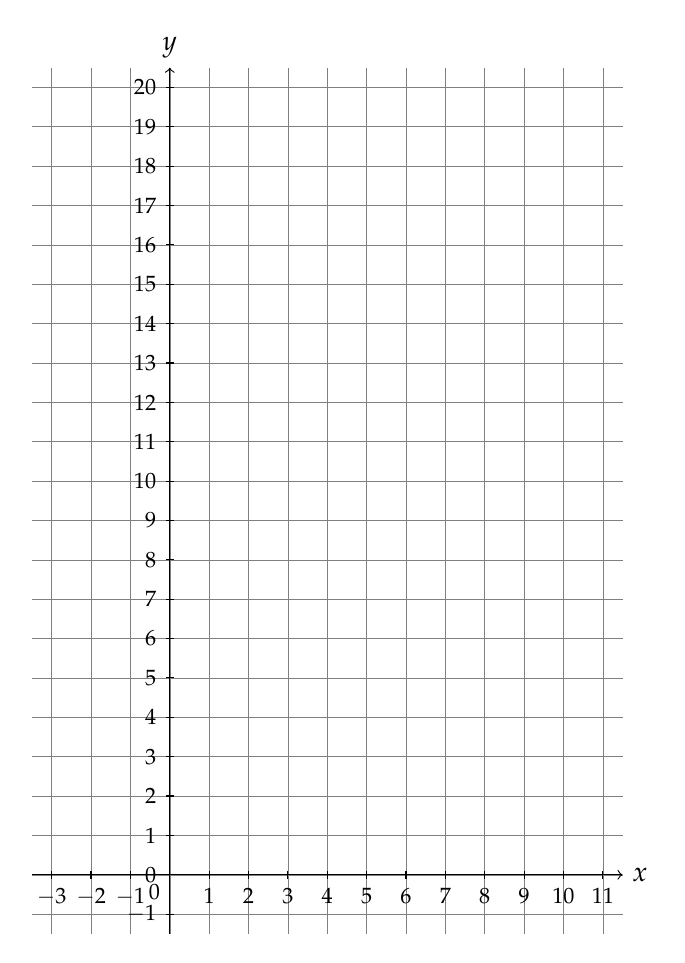
\begin{tikzpicture}[scale=0.5] % Slightly increased scale for better readability, adjusting grid boundaries
        % Grid lines
        \draw[step=1cm,gray,very thin] (-3.5,-1.5) grid (11.5,20.5); % x from -3.5 to 11.5, y from -1.5 to 20.5
        % Axes
        \draw[->] (-3.5,0) -- (11.5,0) node[right] {$x$};
        \draw[->] (0,-1.5) -- (0,20.5) node[above] {$y$};
        % X-axis ticks and labels
        \foreach \x in {-3,-2,-1,1,2,...,11}
            \draw (\x,0.1) -- (\x,-0.1) node[below] {\footnotesize $\x$};
        % Y-axis ticks and labels - ensures 0,1,2 and positive values are shown from a clear starting point
        \foreach \y in {-1,0,1,2,...,20}
            \draw (0.1,\y) -- (-0.1,\y) node[left] {\footnotesize $\y$};
        % Origin label
        \node at (0,0) [below left] {\footnotesize 0};
    \end{tikzpicture}
\end{frame}

% Problem 2
\begin{frame}{Practice Problem 2}
    \begin{tcolorbox}[colback=lightgray,colframe=primary,title=Problem 2]
        \footnotesize
        \[ y = -2(x+1)^2 + 8 \]
    \end{tcolorbox}
\end{frame}

\begin{frame}{Solution to Problem 2 - Analysis}
    \begin{tcolorbox}[colback=lightgray,colframe=accent,title=Solution 2]
        \footnotesize
        For $y = -2(x+1)^2 + 8$, we have $a=-2$, $p=-1$, $q=8$.
        \begin{itemize}
            \item \textbf{Vertex:} $(p,q) = (-1,8)$
            \item \textbf{AOS:} $x = p \implies x = -1$
            \item \textbf{Y-intercept:} Set $x=0$
                \begin{align*}
                    y &= -2(0+1)^2 + 8 \\
                    y &= -2(1)^2 + 8 \\
                    y &= -2 + 8 = 6
                \end{align*}
                Y-intercept: $(0,6)$
        \end{itemize}
    \end{tcolorbox}
\end{frame}

\begin{frame}{Solution to Problem 2 - X-intercepts & Domain/Range}
    \begin{tcolorbox}[colback=lightgray,colframe=accent,title=Solution 2 (Cont.)]
        \footnotesize
        For $y = -2(x+1)^2 + 8$:
        \begin{itemize}
            \item \textbf{X-intercepts:} Set $y=0$
                \begin{align*}
                    0 &= -2(x+1)^2 + 8 \\
                    -8 &= -2(x+1)^2 \\
                    4 &= (x+1)^2 \\
                    \pm\sqrt{4} &= x+1 \\
                    \pm 2 &= x+1
                \end{align*}
                So, $x+1=2 \implies x=1$ and $x+1=-2 \implies x=-3$.\\
                X-intercepts: $(1,0)$ and $(-3,0)$
            \item \textbf{Domain:} $x \in \mathbb{R}$
            \item \textbf{Range:} Since $a=-2<0$, the parabola opens down. $y \leq q \implies y \leq 8$
        \end{itemize}
    \end{tcolorbox}
\end{frame}

\begin{frame}{Solution to Problem 2 - Graphing Grid}
    \centering
    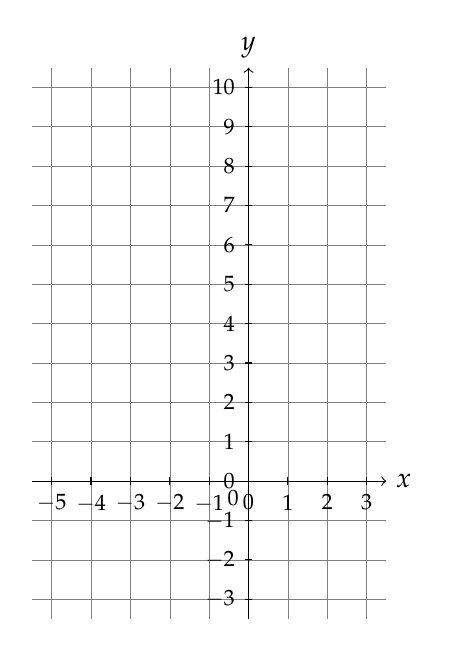
\begin{tikzpicture}[scale=0.5] % Adjusted scale
        % Grid lines
        \draw[step=1cm,gray,very thin] (-5.5,-3.5) grid (3.5,10.5);
        % Axes
        \draw[->] (-5.5,0) -- (3.5,0) node[right] {$x$};
        \draw[->] (0,-3.5) -- (0,10.5) node[above] {$y$};
        % X-axis ticks and labels
        \foreach \x in {-5,-4,...,3}
            \draw (\x,0.1) -- (\x,-0.1) node[below] {\footnotesize $\x$};
        % Y-axis ticks and labels
        \foreach \y in {-3,-2,-1,0,1,2,...,10}
            \draw (0.1,\y) -- (-0.1,\y) node[left] {\footnotesize $\y$};
        % Origin label
        \node at (0,0) [below left] {\footnotesize 0};
    \end{tikzpicture}
\end{frame}

% Problem 3
\begin{frame}{Practice Problem 3}
    \begin{tcolorbox}[colback=lightgray,colframe=primary,title=Problem 3]
        \footnotesize
        \[ y = \frac{1}{2}(x-3)^2 - 2 \]
    \end{tcolorbox}
\end{frame}

\begin{frame}{Solution to Problem 3 - Analysis}
    \begin{tcolorbox}[colback=lightgray,colframe=accent,title=Solution 3]
        \footnotesize
        For $y = \frac{1}{2}(x-3)^2 - 2$, we have $a=\frac{1}{2}$, $p=3$, $q=-2$.
        \begin{itemize}
            \item \textbf{Vertex:} $(p,q) = (3,-2)$
            \item \textbf{AOS:} $x = p \implies x = 3$
            \item \textbf{Y-intercept:} Set $x=0$
                \begin{align*}
                    y &= \frac{1}{2}(0-3)^2 - 2 \\
                    y &= \frac{1}{2}(-3)^2 - 2 \\
                    y &= \frac{1}{2}(9) - 2 \\
                    y &= 4.5 - 2 = 2.5
                \end{align*}
                Y-intercept: $(0, 2.5)$
        \end{itemize}
    \end{tcolorbox}
\end{frame}

\begin{frame}{Solution to Problem 3 - X-intercepts & Domain/Range}
    \begin{tcolorbox}[colback=lightgray,colframe=accent,title=Solution 3 (Cont.)]
        \footnotesize
        For $y = \frac{1}{2}(x-3)^2 - 2$:
        \begin{itemize}
            \item \textbf{X-intercepts:} Set $y=0$
                \begin{align*}
                    0 &= \frac{1}{2}(x-3)^2 - 2 \\
                    2 &= \frac{1}{2}(x-3)^2 \\
                    4 &= (x-3)^2 \\
                    \pm\sqrt{4} &= x-3 \\
                    \pm 2 &= x-3
                \end{align*}
                So, $x-3=2 \implies x=5$ and $x-3=-2 \implies x=1$.\\
                X-intercepts: $(5,0)$ and $(1,0)$
            \item \textbf{Domain:} $x \in \mathbb{R}$
            \item \textbf{Range:} Since $a=\frac{1}{2}>0$, the parabola opens up. $y \geq q \implies y \geq -2$
        \end{itemize}
    \end{tcolorbox}
\end{frame}

\begin{frame}{Solution to Problem 3 - Graphing Grid}
    \centering
    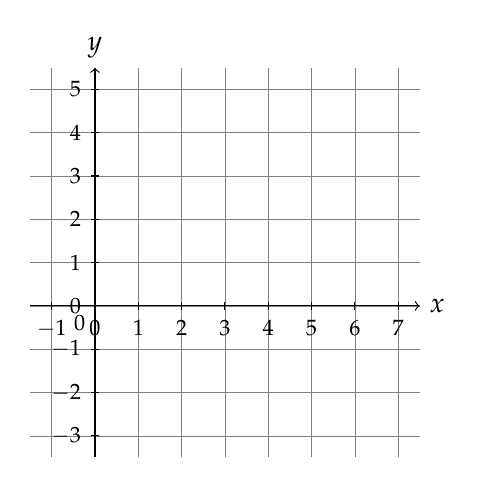
\begin{tikzpicture}[scale=0.55] % Adjusted scale for better fit
        % Grid lines
        \draw[step=1cm,gray,very thin] (-1.5,-3.5) grid (7.5,5.5);
        % Axes
        \draw[->] (-1.5,0) -- (7.5,0) node[right] {$x$};
        \draw[->] (0,-3.5) -- (0,5.5) node[above] {$y$};
        % X-axis ticks and labels
        \foreach \x in {-1,0,1,...,7}
            \draw (\x,0.1) -- (\x,-0.1) node[below] {\footnotesize $\x$};
        % Y-axis ticks and labels
        \foreach \y in {-3,-2,-1,0,1,2,...,5}
            \draw (0.1,\y) -- (-0.1,\y) node[left] {\footnotesize $\y$};
        % Origin label
        \node at (0,0) [below left] {\footnotesize 0};
    \end{tikzpicture}
\end{frame}

% Problem 4
\begin{frame}{Practice Problem 4}
    \begin{tcolorbox}[colback=lightgray,colframe=primary,title=Problem 4]
        \footnotesize
        \[ y = - (x+5)^2 - 1 \]
    \end{tcolorbox}
\end{frame}

\begin{frame}{Solution to Problem 4 - Analysis}
    \begin{tcolorbox}[colback=lightgray,colframe=accent,title=Solution 4]
        \footnotesize
        For $y = - (x+5)^2 - 1$, we have $a=-1$, $p=-5$, $q=-1$.
        \begin{itemize}
            \item \textbf{Vertex:} $(p,q) = (-5,-1)$
            \item \textbf{AOS:} $x = p \implies x = -5$
            \item \textbf{Y-intercept:} Set $x=0$
                \begin{align*}
                    y &= -(0+5)^2 - 1 \\
                    y &= -(5)^2 - 1 \\
                    y &= -25 - 1 = -26
                \end{align*}
                Y-intercept: $(0,-26)$
        \end{itemize}
    \end{tcolorbox}
\end{frame}

\begin{frame}{Solution to Problem 4 - X-intercepts & Domain/Range}
    \begin{tcolorbox}[colback=lightgray,colframe=accent,title=Solution 4 (Cont.)]
        \footnotesize
        For $y = - (x+5)^2 - 1$:
        \begin{itemize}
            \item \textbf{X-intercepts:} Set $y=0$
                \begin{align*}
                    0 &= -(x+5)^2 - 1 \\
                    1 &= -(x+5)^2 \\
                    -1 &= (x+5)^2
                \end{align*}
                Since a square cannot be negative, there are \textbf{No Real X-intercepts}.
            \item \textbf{Domain:} $x \in \mathbb{R}$
            \item \textbf{Range:} Since $a=-1<0$, the parabola opens down. $y \leq q \implies y \leq -1$
        \end{itemize}
    \end{tcolorbox}
\end{frame}

\begin{frame}{Solution to Problem 4 - Graphing Grid}
    \centering
    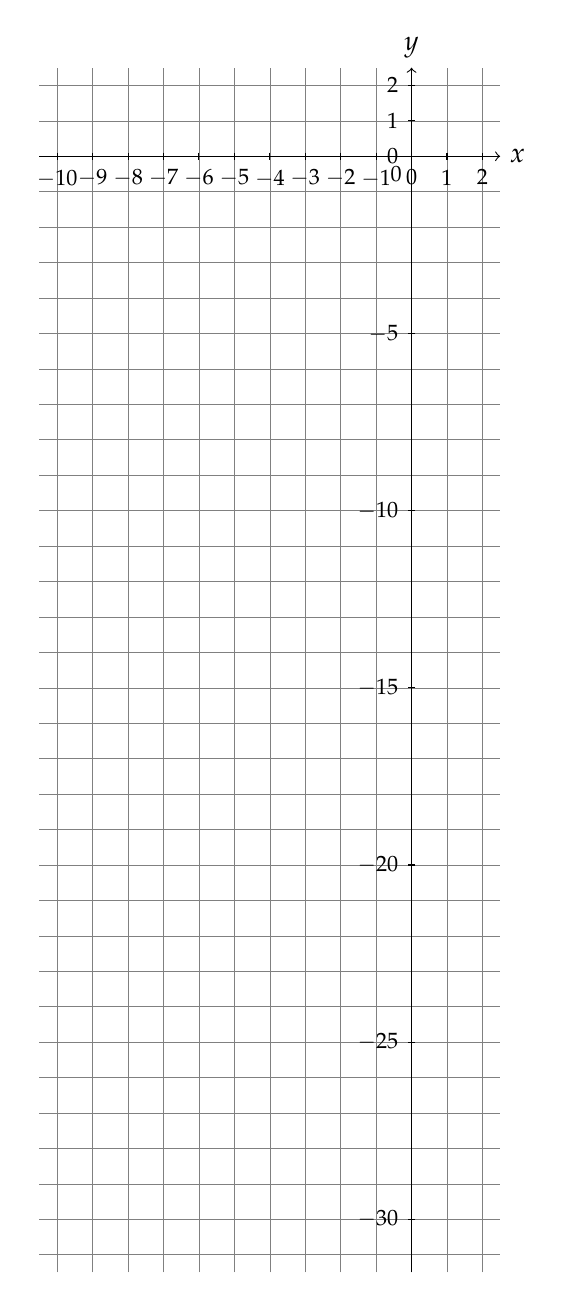
\begin{tikzpicture}[scale=0.45] % Further adjusted scale for large Y range
        % Grid lines
        \draw[step=1cm,gray,very thin] (-10.5,-31.5) grid (2.5,2.5);
        % Axes
        \draw[->] (-10.5,0) -- (2.5,0) node[right] {$x$};
        \draw[->] (0,-31.5) -- (0,2.5) node[above] {$y$};
        % X-axis ticks and labels
        \foreach \x in {-10,-9,...,2}
            \draw (\x,0.1) -- (\x,-0.1) node[below] {\footnotesize $\x$};
        % Y-axis ticks and labels (adjust spacing due to large range)
        \foreach \y in {-30,-25,...,-5,0,1,2}
            \draw (0.1,\y) -- (-0.1,\y) node[left] {\footnotesize $\y$};
        % Origin label
        \node at (0,0) [below left] {\footnotesize 0};
    \end{tikzpicture}
\end{frame}

% Problem 5
\begin{frame}{Practice Problem 5}
    \begin{tcolorbox}[colback=lightgray,colframe=primary,title=Problem 5]
        \footnotesize
        \[ y = 3(x-1)^2 \]
    \end{tcolorbox}
\end{frame}

\begin{frame}{Solution to Problem 5 - Analysis}
    \begin{tcolorbox}[colback=lightgray,colframe=accent,title=Solution 5]
        \footnotesize
        For $y = 3(x-1)^2$, we have $a=3$, $p=1$, $q=0$.
        \begin{itemize}
            \item \textbf{Vertex:} $(p,q) = (1,0)$
            \item \textbf{AOS:} $x = p \implies x = 1$
            \item \textbf{Y-intercept:} Set $x=0$
                \begin{align*}
                    y &= 3(0-1)^2 \\
                    y &= 3(-1)^2 \\
                    y &= 3(1) = 3
                \end{align*}
                Y-intercept: $(0,3)$
        \end{itemize}
    \end{tcolorbox}
\end{frame}

\begin{frame}{Solution to Problem 5 - X-intercepts & Domain/Range}
    \begin{tcolorbox}[colback=lightgray,colframe=accent,title=Solution 5 (Cont.)]
        \footnotesize
        For $y = 3(x-1)^2$:
        \begin{itemize}
            \item \textbf{X-intercepts:} Set $y=0$
                \begin{align*}
                    0 &= 3(x-1)^2 \\
                    0 &= (x-1)^2 \\
                    0 &= x-1 \\
                    x &= 1
                \end{align*}
                X-intercept: $(1,0)$ (This is also the vertex, meaning the parabola touches the x-axis at one point).
            \item \textbf{Domain:} $x \in \mathbb{R}$
            \item \textbf{Range:} Since $a=3>0$, the parabola opens up. $y \geq q \implies y \geq 0$
        \end{itemize}
    \end{tcolorbox}
\end{frame}

\begin{frame}{Solution to Problem 5 - Graphing Grid}
    \centering
    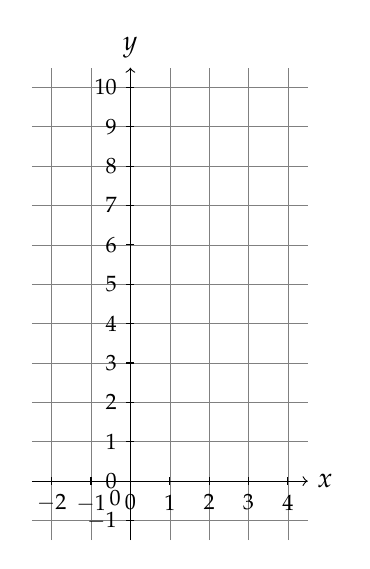
\begin{tikzpicture}[scale=0.5]
        % Grid lines
        \draw[step=1cm,gray,very thin] (-2.5,-1.5) grid (4.5,10.5);
        % Axes
        \draw[->] (-2.5,0) -- (4.5,0) node[right] {$x$};
        \draw[->] (0,-1.5) -- (0,10.5) node[above] {$y$};
        % X-axis ticks and labels
        \foreach \x in {-2,-1,0,1,...,4}
            \draw (\x,0.1) -- (\x,-0.1) node[below] {\footnotesize $\x$};
        % Y-axis ticks and labels
        \foreach \y in {-1,0,1,2,...,10}
            \draw (0.1,\y) -- (-0.1,\y) node[left] {\footnotesize $\y$};
        % Origin label
        \node at (0,0) [below left] {\footnotesize 0};
    \end{tikzpicture}
\end{frame}

\end{document} 